\documentclass[ notitlepage, numerical, 11pt]{revtex4-1} % style for Physical Review B and AJP are similar
\usepackage{float}
\usepackage{amsmath}
\usepackage{appendix}
\usepackage{graphicx} 
\usepackage{url}
\usepackage{breakurl}
\usepackage[breaklinks]{hyperref}
\def\UrlBreaks{\do\/\do-}



\usepackage{sverb}

\begin{document}

\title{Physics of Non-Volatile Digital Data Storage Technologies}
\author{Tenzin Rigden}
\affiliation{Carleton College, Department of Physics, Northfield, MN 55057}
\date{\today}
\begin{abstract}
Data storage technologies have become increasingly important as more and more of our lives are being stored digitally in our phones and computers and the need for higher density and larger capacity data storage techniques increases. In this paper, I will discuss the physics behind techniques used today such as optical storage, flash storage, and magnetic storage and the advances they have made to increase their storage capacities. I will then discuss Holographic Data Storage, a novel technique that has the potential to increase storage capacities past what is currently available.

\end{abstract}

\maketitle
\section{Introduction}
Computers and phones have become such a ubiquitous part of our lives that it is becoming more and more difficult to live without them. Just as important as these devices themselves are their contents. Your pictures, music, videos, papers, and more are all stored digitally on the devices. As more and more of our lives are recorded digitally, it has become increasingly important to find new ways to either expand our current data storage technologies or find new ones. On a fundamental level, a computer stores everything in a series of 1s or 0s called bits. In this binary system, 1 represents a ``true" state while a 0 represents a ``false" state. By using this binary system, it is possible to represent numbers as a sequence of 1s and 0s where each digit starting from the right represent an increasing power of 2 starting with $2^0$. For example, the number 13 can be represented as 1101 so we get, from the right, 1*$2^0$ + 0*$2^1$ + 1*$2^2$ + 1*$2^3$ which adds up to 13. Since we can represent numbers, we can use these numbers to represent other characters. One method is to use the American Standard Code for Information Interchange (ASCII) encoding system which was first published in 1963, an ASCII table can be seen in the appendix. ASCII encodes 128 characters that include letters, both lower case and capital, numbers, and other special characters into 7 bit integers. For example, the capital letter T corresponds to the 84th character and thus in binary can be represented as 01010100. A series of these binary numbers can be used to represent text.


Now that we know we can use binary to represent text, we can look at how we can physically store these 1s and 0s. One of the earlier methods was to use punch cards with holes and not holes representing 1s and 0s respectively. In this paper, I will talk about modern techniques that are currently being used for non-volatile memory, data that will not be lost if the device does not have power. I will discuss in order of increasing storage capacity. That means beginning with optical disks, continuing on to flash memory storage, and then magnetic data storage. Lastly, I will talk about holographic data storage which promises to  increase storage density and capacity.





\section{Optical Disk Storage}
\begin{figure}[H]
\centerline{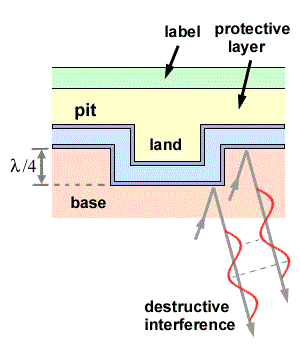
\includegraphics[scale=.9]{cdRom.png}}
\caption{ This is a cross-sectional view of a CD-ROM where there a pit signifies a $\lambda/4$ depth meaning when a laser shines over a change from land to pit or vice versa, destructive interference will take place signifying a bit value of 1 \cite{cdCross}.}
\label{cdRom}
\end{figure}

Optical disks are a form of data storage that use the grooves in the disk to store data. They have been commonplace in the United States since their invention in 1958 \cite{memory}. While optical disks are not used for storing data directly from the computer, they are used to archive or transfer data between machines. For optical disks, data is recorded and read using a laser beam. To record data onto a writable disk, a laser beam is shone on the reflective surface creating a pit, a tiny indentation, with a depth of the wavelength of the laser divided by 4. As seen in Fig. \ref{cdRom}, to read data, a very low power laser is shone on the disk and the reflected signal is converted to an electrical signal using a scanning photo detector. A binary value of 1 is recorded when there is a change in the surface depth due to switching to a pit to land or vice versa, and a 0 is interperted as when there is no change in the surface depth. When the laser is shone over an intersection between a pit and a land, there will be light reflected from the pit and the land resulting in two beams \cite{memory}. These two beams will then destructively interefere back at the photo-diode. To see how they interfere, we can look at it mathematically. 


\subsection{Destructive Interference}
When two waves arrive at the same point the superpostion of those waves creates a new wave. Interference depends on the superposition of the waves and certain conditions. In our example, since we have a laser beam being split into two beams, we have coherent light (there is a constant phase difference between two beams), and both beams have the same frequency. Thus, we can define the electric field of the two beams as


\begin{align}
\begin{split}
\vec{E}_{1} = \vec{E}_{01} cos(k s_1-\omega t + \phi_1) \\
\vec{E}_{2} = \vec{E}_{02} cos(k s_1-\omega t + \phi_1),
\end{split}
\label{eRefInf}
\end{align}
where $ \vec{E}_{01}$ and $ \vec{E}_{02}$ are the amplitudes for the wave, $k$ is defined as $\frac{2\pi}{\lambda}$, $s_1$ and $s_2$ are defined as distance traveled by each beam, and $\phi_1$ and $\phi_2$ are the phases of the beams at t = 0 at their source \cite{optics}. Since we have the same source for both of our beams, the amplitudes and the phase at t = 0 are the same. Next, the superposition of these two waves at a point $P$ is 

\begin{equation}
\vec{E}_{P} = \vec{E}_{1} + \vec{E}_{2}.
\label{ePInf}
\end{equation}

The measurement of the effect of this wave on our eyes or a detector depends on the energy of the light beam. The irradiance, $I$, is the time average of the square of the wave amplitude and is is used to measure effects of waves \cite{optics}. The time average of the irradiance is done by the detector; our eye for example has an averaging time of 1/30 of a second. The irradiance is defined as 

\begin{equation}
I = \epsilon_0 c<\vec{E}_{P}\cdot \vec{E}_{P}>,
\label{iInf}
\end{equation}
where $\epsilon_0$ is the vacuum permittivity and $c$ is the speed of light \cite{optics}. By subbing in Eq. \ref{ePInf} for $\vec{E}_{P}$ and simplifying we get 
\begin{equation}
I = \epsilon_0 c<\vec{E}_{1}\cdot \vec{E}_{1}+\vec{E}_{2}\cdot \vec{E}_{2}+2\vec{E}_{1}\cdot \vec{E}_{2}>.
\label{iInf2}
\end{equation}
The first two terms correspond to the irradiances of the individual beams while the third term corresponds to the interaction between the waves and is the interference term, $I_{12}$ \cite{optics}. Thus, $I$ can be rewritten as 
\begin{equation}
I = I_1 + I_2 + I_{12}.
\label{iInf3}
\end{equation}The interference term, $I_{12}$, by using a trigonemtric identity and simplifying, can be written as 

\begin{equation}
I_{12} = 2\sqrt{I_1 I_2}<cos\delta>,
\label{iInf2}
\end{equation}
where $\delta$ is the phase difference and is defined as 
\begin{equation}
\delta = k(s_2 - s_1) +\phi_2 -\phi_1.
\label{delta}
\end{equation}
Finally, we can write $I$ as 
\begin{equation}
I = I_1 + I_2 +  2\sqrt{I_1 I_2}<cos\delta>.
\label{finalI}
\end{equation}
Destructive interference will yield a minimum value when $cos\delta$ is -1. In our case, since the beams have the same source, the laser, $I_1$ = $I_2$ and $\phi_1$ =  $\phi_2$, so $\delta$ will be 0 when the path length difference between the beams is $\frac{(2m+1)\lambda}{2}$ where m is an integer. Returning to our CD, since the pit has a depth of $\lambda/4$, the light reflected off of the pit will have a path length difference of $\lambda/2$ relative to the light reflected off of the land. This means that $\delta$ is $\pi$ so $cos\delta$ is -1. So $I$ becomes
\begin{equation}
I = I_1 + I_1 - 2\sqrt{I_1 I_1} = 0.
\label{finalI2}
\end{equation}
This means at the cliff between a land and a pit, the two reflected beams will completely destructively interfere and no light will be reflected to the photo diode, which is then recorded as a 1. When there is no change in the surface depth, the light reflects back with no phase difference and is recorded as a 0 by the photo-diode \cite{memory}.

\subsection{Disk Types and Layers}
Optical Disks come in a few different styles: Compact Disk ROM (CD-ROM), CD-Recordable (CD-R), and Digital Versatile Disk (DVD). These disk technologies are written sequentially in a continous spiral track eminating from the middle out, the distance between each track is called the pitch. A CD-ROM is a disk that is only readable and is used for things such as installation of programs. Since it is only written once in the factory, a glass master disk is created using a high intensity laser. Liquid polycarbonate is inserted into the master disk to create a copy which is then covered with a reflective layer and then a protective layer over that. 
A CD-R is slightly different because it needs to be writable once outside of the factory. This is done by having a paint layer and reflective layer below the protective layer, Fig. \ref{cdR}. The painted layer is initially transparent and permantly becomes dark to simulate a pit when impacted by a high-intensity laser. This can then be read by a lower intensity laser that does not cause the painted layer to turn dark.



\begin{figure}[H]
\centerline{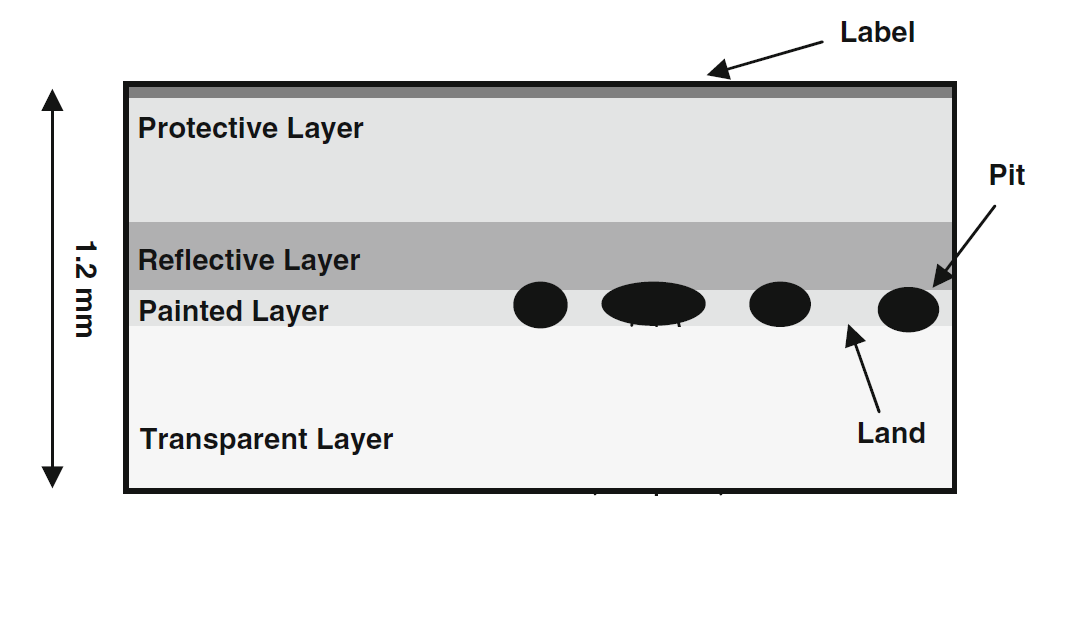
\includegraphics[scale=.45]{cdR.png}}
\caption{In this cross sectional view of a CD-R, the painted layer, if shone on by a high intensity laser will develop dark spots simulating pits \cite{memory}.}
\label{cdR}
\end{figure} 

\subsection{Rayleigh's Criteron due to Diffraction}

While CDs are useful and easy to carry around, their size was limited to only 700 MB until the early '90s when demand for higher storage capacities meant that the disk had to change. Since the data bits are stored in the pits and lands, the way to increase storage density was to decrease their size and also place tracks closer to each other by decreasing their pitch. However, these values can only be decreased to a certain point due to diffraction. Diffraction is the phenomenon where light that propagates through an opening interferes with itself causing a diffraction pattern.
\begin{figure}[H]
\centerline{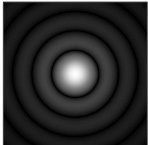
\includegraphics[scale=1.5]{220px-Airy-pattern.jpg}}
\caption{The airy disk created by a diffraction limited circular aperture lens laser. The rings are due to the bessel function of the first order \cite{airyDisk, optics}.}
\label{airy}
\end{figure} 
For lasers which use a circular aperture, the opening through which light travels, the diffraction pattern produced is called an Airy Disk (Fig. \ref{airy}), with the bright circles representing maxima and the dark circles representing minima. The type of diffraction applicable here is Fraunhofer diffraction which is used for far field, larger distance to observation point. To model this, a lens is placed after the aperture and focal distance, $f$, from the observation point such that the observation point observes the light as if it were an infinite distance away, as seen in Fig \ref{fraunD} for a single slit aperture.

\begin{figure}[H]
\centerline{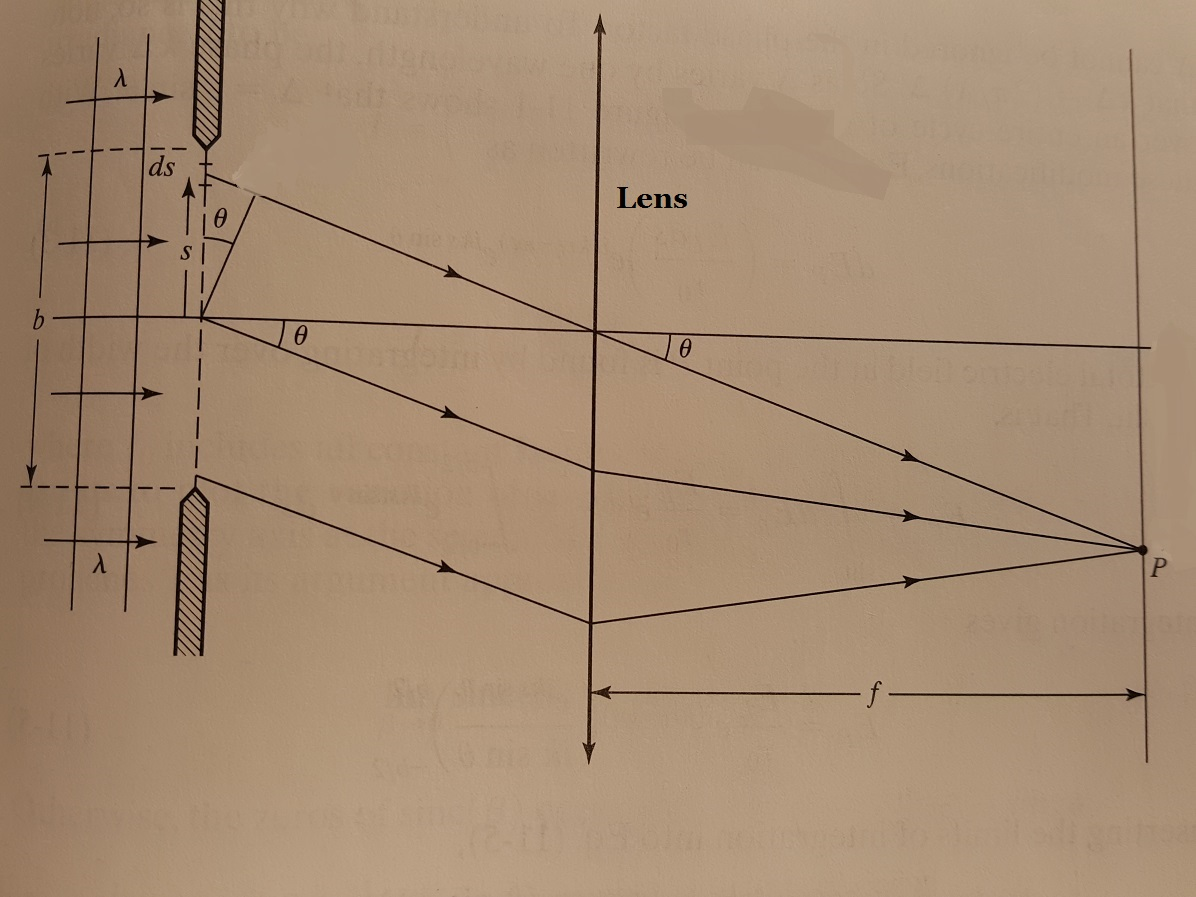
\includegraphics[scale=.2]{fraunD.jpg}}
\caption{A basic setup for a observing Fraunhofer diffraction at point p due to a single slit where b is the length of the aperture, $\lambda$ is the wavelength of lgith, $f$ is the focal length of the lens \cite{optics}.}
\label{fraunD}
\end{figure} The Airy Disk shape can then be derived by starting with the electric field at point p through a circual aperture which can be found by 
\begin{equation}
E_p = \frac{E_A}{r_0}e^{i(k r_0 -\omega t)}\iint \limits_{Area} e^{i s k sin\theta} dA,
\label{EP}
\end{equation}
where $E_A$ is a constant factor that determines the strength of the electric field in the aperture, $k$ is the same as before $\frac{2\pi}{\lambda}$, $dA$ is an elemental area of the aperture as seen in Fig \ref{aperture}, $s$ is the radial distance from the center of the aperture to the $dA$, $\theta$ is the angle of the optical path relative to the axis orthogonal to the aperture, and $r_0$ is the optical path length to the point P \cite{optics}. 

We can write $dA$ as $xds$ where $x$ is $2\sqrt{R^2 - s^2}$ and $R$ is the aperture radius. Eq \ref{EP} then becomes 
\begin{equation}
E_p = 2\frac{E_A}{r_0}e^{i(k r_0 -\omega t)}\int_{-R}^R e^{i s k sin\theta}\sqrt{R^2 - s^2}ds.
\label{EP2}
\end{equation}
Next by making the following substitutions $v = \frac{s}{R}$ and $\gamma = kRsin\theta$, $E_P$ can be rewritten as
\begin{equation}
E_p = 2\frac{E_A R^2}{r_0}e^{i(k r_0 -\omega t)}\int_{-1}^1 e^{i \gamma v}\sqrt{1 - v^2}dv.
\label{EP3}
\end{equation}
\begin{figure}[H]
\centerline{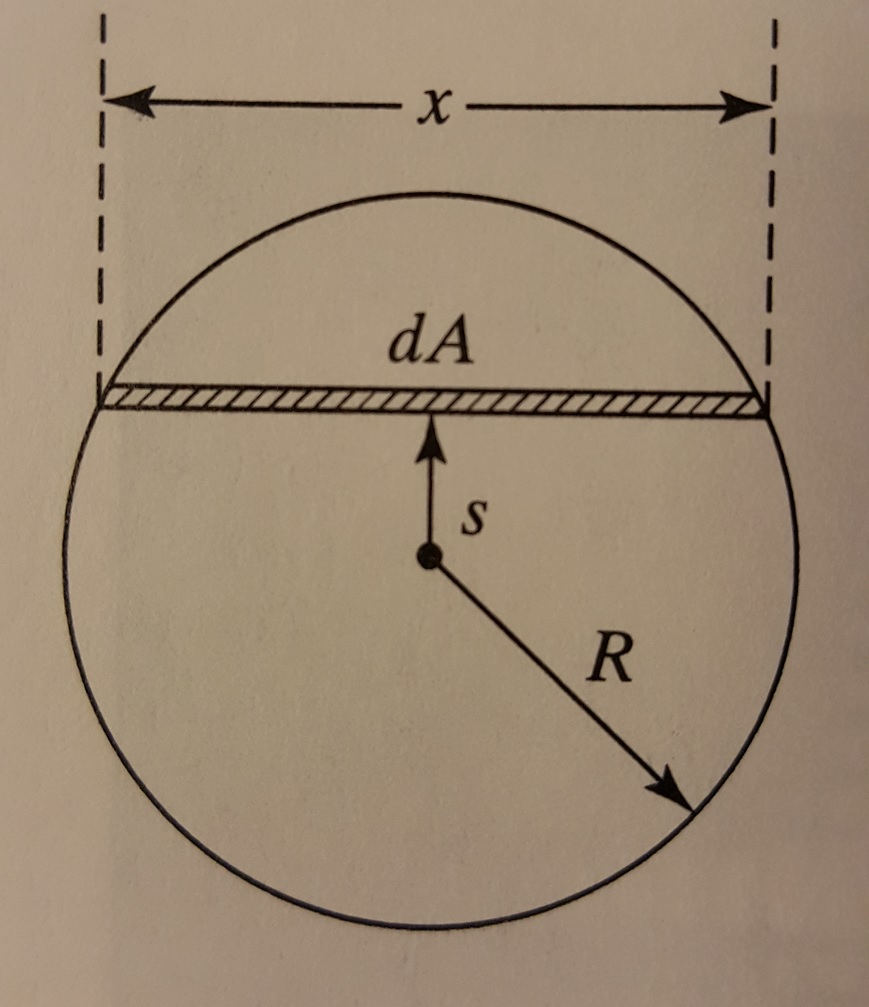
\includegraphics[scale=.20]{bessel.jpg}}
\caption{In calculating Electric field at a point past the aperture, you need to integrate over the area of the aperture. One way to do so is above.\cite{optics}.}
\label{aperture}
\end{figure}The integral on the right side is known to be
\begin{equation}
\int_{-1}^1 e^{i \gamma v}\sqrt{1 - v^2}dv = \frac{\pi J_1(\gamma)}{\gamma},
\label{bessel}
\end{equation}
where $J_1(\gamma)$ is the first-order Bessel function of the first kind and can be represented by the infinite series \cite{optics}
\begin{equation}
J_1(\gamma) = \frac{\gamma}{2} - \frac{(\gamma /2)^3}{1^2 *2} + \frac{(\gamma /2)^5}{1^2 *2^2 *3} - .
\label{besselSeries}
\end{equation} 
Finally, the irradiance at point P can be written as 

\begin{equation}
I =  I_0(\frac{2J_1 (\gamma)}{\gamma})^2,
\label{iBessel}
\end{equation} 
where $\gamma = 1/2 k D sin\theta$, and $I_0$ is made up of all the other constants and is the irradiance at the principle maximum \cite{optics}. This function is what causes the light dark patterns in the Airy disk. In addition, the irradiance of the 2nd maximum as a ratio of $I_0$ is 0.0175. Because the principle maxiumum is so much larger than the 2nd, two point sources are considered resolvable when the principle maximum of one source overlaps with the first minimum of the other as in Fig. \ref{criterion} b. This is known as Rayleigh's Criterion. To create an equation for this criterion, we will need to know when the irradiance first becomes 0 and that distance from the center is the minimum resolvable distance. 
\begin{figure}[H]
\centerline{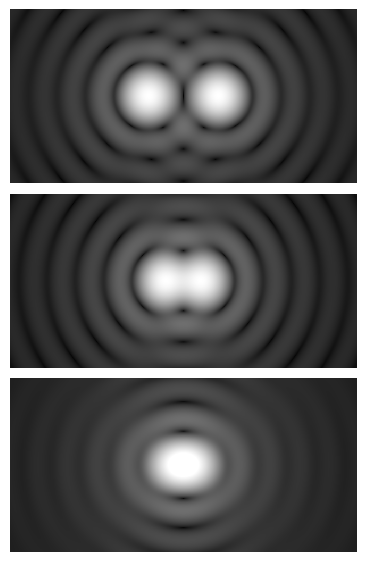
\includegraphics[scale=.45]{criterion.png}}
\caption{The top image shows two resolvable images, the middle image shows Rayleigh's critereon where the first fringe appears over the max of ther other image, and the bottom image shows them being not resolvable \cite{rayleigh}.}
\label{criterion}
\end{figure} 

The irradiance first becomes 0 when $\gamma = 3.832$ \cite{optics} so 
\begin{equation}
\gamma = (\frac{k}{2})Dsin\theta = 3.832 
\label{gamma}
\end{equation} 
If the distance between the lens and aperture is zero, the resolvability of an object is due to the diffraction described above. Using the small angle approximation we get the minimum angular separation, $\delta\theta_min$ as 
\begin{equation}
\delta\theta_min = \frac{1.22\lambda}{D},
\label{thetaMin}
\end{equation} where $D$ is now the diameter of the lens. The product of $\delta\theta_min$ and the distance to the screen, $f$, is the minimum resolvable distance, d, which is
\begin{equation}
d = f\frac{1.22\lambda}{D},
\label{minDF}
\end{equation}
where $f$ is the focal length of the lens. Finally, $f/D$ can be re-written as $1/NA$ where $NA$ is the numerical aperture and indicates the resolving power of a lens. Subbing this into Eq. \ref{minDF}, we get Rayleigh's criterion \cite{memory}.
\begin{equation}
d = \frac{1.22\lambda}{2NA}.
\label{rayleigh}
\end{equation}
If all other optical instruments are perfect, $d$ is the smallest resolvable distance between two objects. To read a CD a laser wavelength of 780 nm is used along with a numerical aperture of 0.45 which yields a minimum resolvable distance of 1.06 $\mu$m. In practice, the minimum resolvable distance for the laser in a CD is 1.6 $\mu$m. As seen in Fig \ref{comparison}, this yields a pit length of 800 nm, a pit width of 600 nm, a pitch of 1.6 $\mu$m, and a storage density of 0.9 Gb/in$^2$ with 700 MB total storage per disk \cite{wikiHolo}). To decrease the minimum resolvable distance, and consequently decrease pit size and pitch, the numerical aperture must be increased and the wavelength of light decreased. This is what DVDs do.

\begin{figure}[H]
\centerline{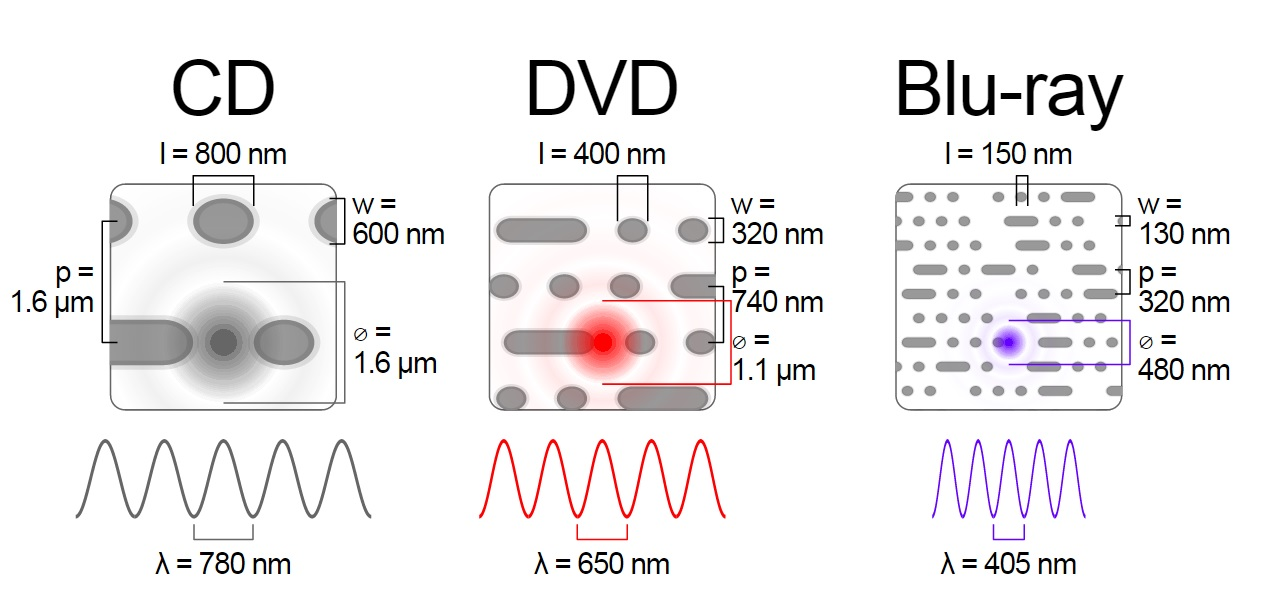
\includegraphics[scale=.55]{comparison.jpg}}
\caption{A comparison of the wavelength of light used, pit length, pit width, pitch, and the minimum resolvable distance for a CD, DVD, and Blu-Ray. The smaller dimensions all around increased the storage capacity of DVDs and then Blu-ray disks. \cite{wikiHolo}.}
\label{comparison}
\end{figure} 
For DVDs, a laser wavelength 650nm and numerical aperture of 0.6 is used. The minimum resolvable distance was decreased to 1.1 $\mu$m and the pit length, pit width, and pitch were all reduced to 400 nm, 320 nm, and 740 nm respectively. This meant that more pits could be packed along the track itself since the pit length was reduced. Also, since the pitch and pit width were reduced, tracks could be placed closer together further increasing density, up to 2.2 Gb/in$^2$ \cite{wikiHolo}. Another innovation that allowed storage of up to 8.5 GB per disk was the ability to have two different recording layers: a semi reflective layer at half the depth of the disk and a fully reflective layer at near the full depth of the disk \cite{memory}. 
The different layers can be read by changing the focus depth of the laser. Additionally, instead of having a protective layer on one side of the disk, as seen in Fig. \ref{DVD} you can put another disk on it to double the capacity again. However, this requires manualy flipping the disk to access the other half of the data. By being double sided and having a double layer, DVDs can achieve storage of 17 GB per disk \cite{memory}.
\begin{figure}[H]
\centerline{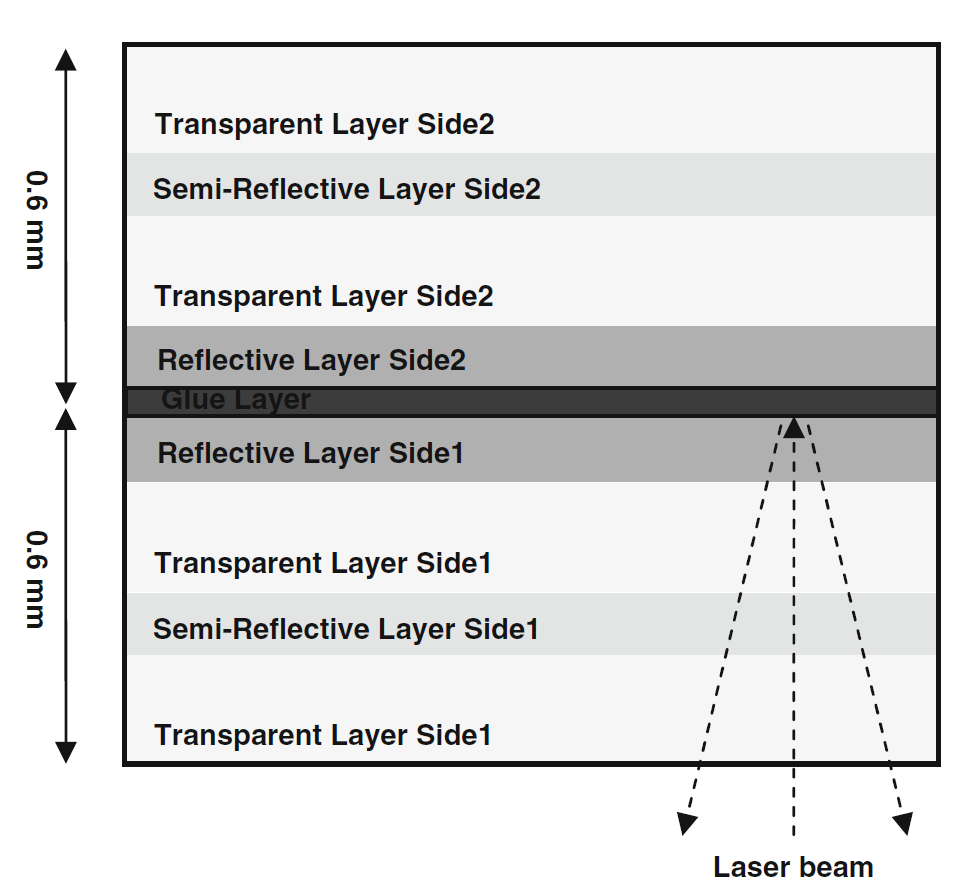
\includegraphics[scale=.45]{DVD.png}}
\caption{This is a cross-section of a double-sided and dual layer DVD. The pit and land information is stored at the two reflective and semi-reflective layers. The layer in which the laser is reading from is selected by focusing the laser to for that layer depth. To access the other side of the DVD, it must be physically removed from the player and re-placed upside down \cite{memory}.}
\label{DVD}
\end{figure}

A more recent innovation in storage of optical disks was the invention of the Blu-Ray disk. Blu-ray disks use a much shorter wavelength light to increase capacity. Blu-ray uses 405 nm light which allows the pit length, pit width, and the pitch to be reduced to 150 nm, 130 nm, and 320 nm respectively. This allows for a storage density of 14.7 Gb/in$^2$ to be achieved and total storage capacity of 25 GB \cite{memory}. The difficulty in creating a stable blue semi-conductor laser is why we did not skip DVDs to Blu-Ray..

 


\subsection{Laser Read System}

The implentation of the laser system used to read the data from the disk can be seen in Fig. \ref{cdPlay}. After the laser source is collimated by the lens to produce a parallel beam, it encounters the polarizing prism. Before we talk about the prism, we need to talk about polarization in the context of light. Light is an electromagnetic wave meaning it has an electric field component and a magnetic field component that are both orthogonal to the direction of propagation. 
\begin{figure}[H]
\centerline{\includegraphics[scale=.8]{cdPlay.png}}
\caption{This is the laser read system set up that corrects depth errors with the positioning coil making sure that the focus of the laser is exactly at the disk surface. It also contains a polarizing beam splitter used to direct the beam to reflect off of the disk and shine onto the photodiode detector\cite{hyper}.}
\label{cdPlay}
\end{figure} 
The polarization of light is the orientation of the electric field. Unpolarized light is light that has random orientations while linearly polarized light is light that has the electric field oscillating in one dimension. A quarter-wave plate is a device that has a fast axis and a slow axis such that when linearly polarized light passes through it, the quarter-wave plate applies a 90 degree phase retardation between the component of the E-field on the fast axis vs the slow axis \cite{optics}. As seen in Fig. \ref{circular}, this creates an electric field that traces out an ellipse while propagating.
\begin{figure}[H]
\centerline{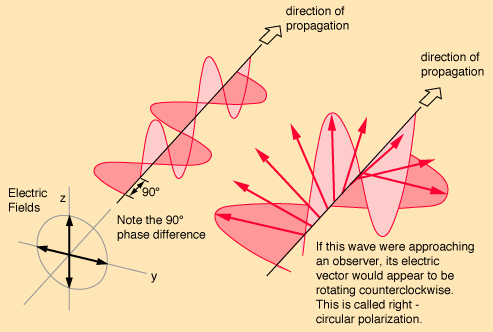
\includegraphics[scale=1]{polcir.png}}
\caption{Circular polarized light on the left with a 90 degree phase difference between two electric fields which makes the tip of electric field trace out a circle while propagating\cite{wikiPic}.}
\label{circular}
\end{figure} 

As seen in Fig. \ref{prism}, the polarizing beam splitter allows the polarization parallel to the plane of incidence of the beam through while reflecting the polarization perpendicular to the plane. This is known as P and S polarization, respectively. The linearly polarized light then goes through a quarter-wave plate circularly polarizing it. Next the light is reflected off of the disk back to the quarter-wave plate. Since it was reflected, the direction of the circular polarization is flipped, so when it passes back through the quarter-wave plate, it becomes linearly polarized but with an orientation orthogonal to the one it had after it passed through the beam splitter. This means that when it comes back through the beam splitter, it will be reflected towards the photodiode. 
\begin{figure}[H]
\centerline{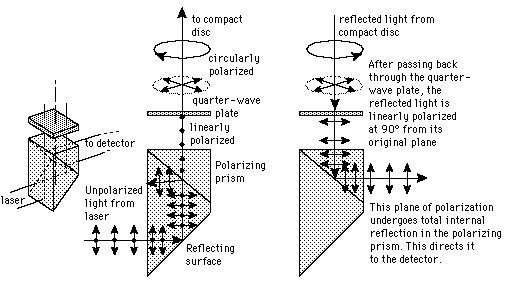
\includegraphics[scale=1.1]{prism.png}}
\caption{Unpolarized light enters the beam-splitter. The polarizing beam splitter allows the P-polarization, parallel to the plane of incidence, through while reflecting the S polarization which is perpendicular to the plane. Then, passing it through a quarter-waveplate circularly polarizes it and the reflection off of the disk reverses the direction of the polarization. Finally, the now S polarization is reflected by the beam-splitter towards the photodiode, not seen \cite {hyper, optics}.}
\label{prism}
\end{figure} 

The last part of the system is the focusing lens and positioning coil. If the laser is not properly focused onto the surface of the disk, the beam will be larger and the minimum resolvable distance will increase meaning that the size of the beam will be large enough that it might overflow into other tracks and not read properly. To prevent this, the laser light is reflected off the disk and then goes through the focusing cylindrical lens which is then shone on to the 4 component photodiode, seen in Fig. \ref{focus}. Since a cylindrical lens focuses in one axis, there will only be one distance from the lens to the source image (the disk surface in this case) that will cause the laser beam to be circular, Fig. \ref{focus2}. If the image distance is too far or too close, the beam will appear oval shaped and the photodiodes will create an error voltage that drives a coil to reposition the lens so it is properly focused. If the beam is too close, the A and C components in the photodiode will be larger than the B and D components so the difference amplifier will send a positive current to the positioning coil that will re-adjust it. If the beam is too far, the B and D components are larger than the A and C components causing a negative current to be sent to the positioning coil. Though disks have been increasing in capacity, they still can not compete with flash and hard disk drives (HDDs).




\begin{figure}[H]
\centerline{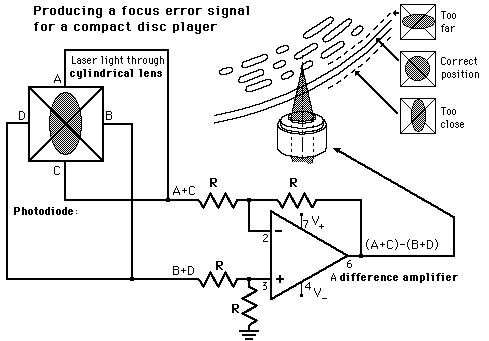
\includegraphics[scale=.7]{focus.png}}
\caption{The positioning coil uses a cylindrical lens that causes the laser's focus point to occur at the disk surface because if it was not the reflected image on the diode would not be circular and the difference amplifier would send a current to the positioning coil that would move to adjust the position of the lens. \cite {hyper}.}
\label{focus}
\end{figure} 

\begin{figure}[H]
\centerline{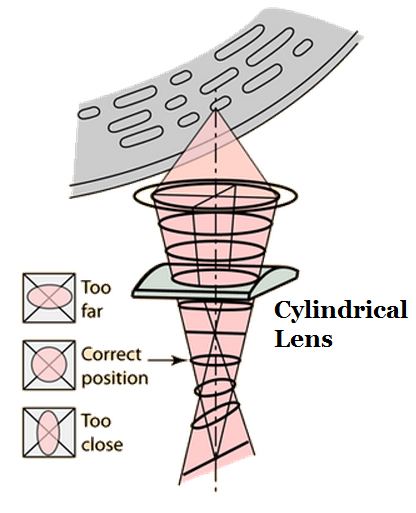
\includegraphics[scale=.5]{rayDiagram.png}}
\caption{A ray diagram of the laser being refracted by the cylindrical lens so that there is only one depth where the produced image is a perfect circle \cite {hyper}.}
\label{focus2}
\end{figure} 

\section{Flash Memory}
Flash memory has been becoming popular recently as a replacement for hard drives due to their speed. One of the most, if not the most, important device in flash memory and modern computing and as a whole is the transistor. A transistor is able to take in a circuit input and act as a switch turning other circuits on or off without any moving parts. This ability to switch a circuit off and on will prove crucial in saving bits of memory.

\subsection{Semiconductors}
To explain how transistors work, first we need to explain what a semiconductor is since a transistor is a semiconductor device. A bandgap diagram is useful in describing semiconductors. Band structure represents the specific energy levels that electrons can occupy due to quantum mechanics. However, only the valence band and the conduction band are relevant when discussing conductivity. The valence band is the highest energy levels that electrons can occupy at absolute zero temperature while the conduction band is where electrons can move freely. As seen in Fig. \ref{bandGap}, the conductor is any material that does not have a bandgap between the valence band and conduction band or the valence band is not filled meaning electrons can move freely. An insulator is any material whose conduction band is separated by a large band gap from its valence band. This means that the valence electrons can not easily move to its conduction band and thus are not free too move. Lastly, a semiconductor is any material whose conduction band is separated from the valence band by a band gap small enough that thermal or optical fluctuations can excite electrons to the conduction band \cite{purcell}.


\begin{figure}[H]
\centerline{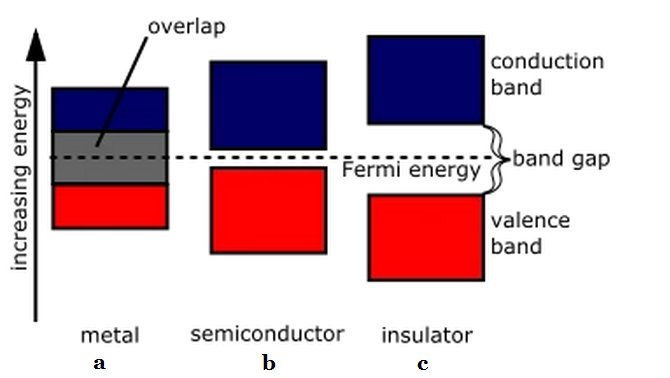
\includegraphics[scale=.6]{bandGap.png}}
\caption{Metals/conductors, a, are materials where their valence electrons are free to move in the overlapping conduction band. Insulators, c, are materials which have their valence electrons are unable to move in their valence band and are unable to easily access the conduction band. Semiconductors, b, are materials which have their electrons unable to move in their valence band, but are easily exicted into the conduction band where they can carry current.}
\label{bandGap}
\end{figure}


Most commercial applications of semiconductors use impurity semiconductors. Impurity semiconductors are materials that gain different properties than pure semiconductors by adding an impurity, dopant, to the material. For example, say we have silicon with 4 valence electrons where each valence electron is shared with another silicon atom to create a tetrahedron. Then if we replace one of those silicon atoms with a phosphorus atom with 5 valence electrons, 4 of the 5 valence electrons will be shared with the 4 nearby silicon atoms, but the last one is loosly bound to the phosphorus. At room temperature, thermal energy is enough to release it from this loosly bound state and it becomes a conduction electron. This is called n-type doping. If instead of adding an element with 5 valence electrons and instead added one with only 3, we would then have one less electron than its pure state which is represented as a hole.This is called p-type doping \cite{purcell}.

A simple example of a semiconductor device is the pn junction diode. This device is created when a p-type semiconductor comes in contact with an n-type semiconductor. Since p-type materials have a higher concentration of holes than the n-type, holes diffuse across to the n-type material while electrons diffuse the other way; this is the diffusion current. The holes and electrons that diffuse then recombine in the n-type and p-type material respectively. This creates a depletion zone at the intersection of the two materials. The diffusion and recombination also creates a net positive charge in the p-type material and a net negative charge in the p type material creating an electric field towards the p-type. The diode is in equilibrium when the drift current and diffusion current are equal \cite{thermo}.

The special property of a PN junction is that current is only allowed to flow in one direction. In Fig. \ref{pnJunction}a, the orientation of the battery applies a clockwise current pushing holes from the p type and electrons from the n type towards the interface where they combine and produce heat. So the diode loses electrons and holes at the interface due to recombination, however the current pulls electrons from the p type resupplying the p type with holes. The converse happens in the n type so a current can flow indefinitely. This is known as forward bias. In Fig. \ref{pnJunction}b the opposite orientation of the battery applies a counter-clockwise current directing the holes in the p type and the electrons in the n type to flow away from the interface. The flow of electrons and holes away from the interface continues until the local electric field produced is strong enough to oppose the applied potential, causing the current to stop; this is known as reverse-bias \cite{thermo}.


\begin{figure}[H]
\centerline{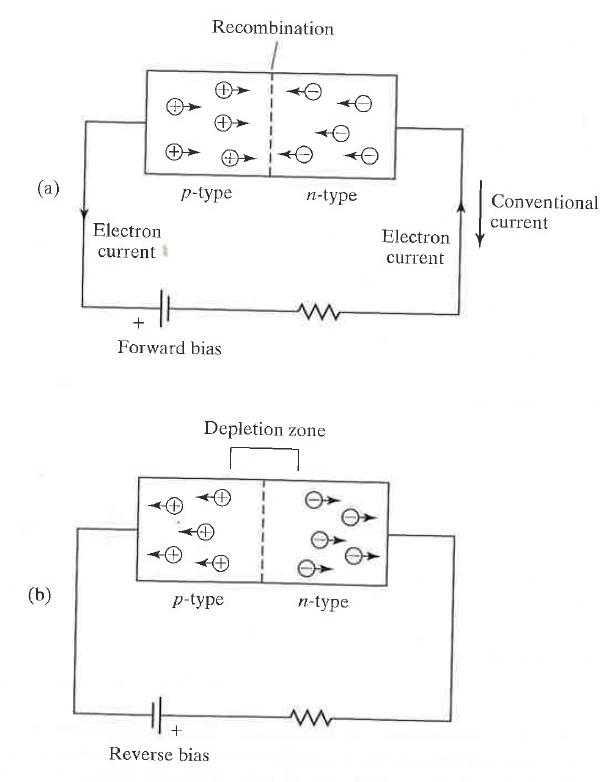
\includegraphics[scale=.5]{pnJunction.png}}
\caption{This is a diagram of a pn junction diode with current in different directions. In the clockwise current in a, the holes and electrons are constantly refreshed due to the applied potential, and the current can continuously flow. In the counterclockwise current, b, the applied potential increases the depeletion zone until the local electric field cancels out the applied potential and stops the flow of current.}
\label{pnJunction}
\end{figure}



\subsection{Transistors}
So now that we know what p-type and n-type doped semiconductors and pn junction diodes are, we can now talk about transistors. While there are many different types of semiconductors, the one that flash memory uses is the metal oxide semiconductor field effect transistor (MOSFET). A MOSFET, as seen in Fig. \ref{mosfet}a consists of a p-type silicon with two n-type regions, one on each side as a source and drain. There is also a metal gate separated from the semiconductor by an insulating oxide layer in the middle. When no voltage is applied to the gate as seen in Fig. \ref{mosfet}a, the MOSFET acts as two pn diodes, and so any voltage difference between the source and drain will reverse-bias one of the two pn diodes so no current will flow. However, if a positive voltage is applied to the gate, the positive charge attracts electrons and repels holes as in Fig. \ref{mosfet}b. If the voltage applied to the gate is above a certain threshold of around 1 Volt, a thin layer of electrons will be formed under the oxide. Also known as the inversion layer, this creates a conducting channel between the source and drain, and the p-type silicon acts as an n-type material at the oxide layer due to the extra electrons allowing current to flow between the source and drain. This change created by the field from the gate is why it is called a field effect transistor \cite{modernPhysics}.

\begin{figure}[H]
\centerline{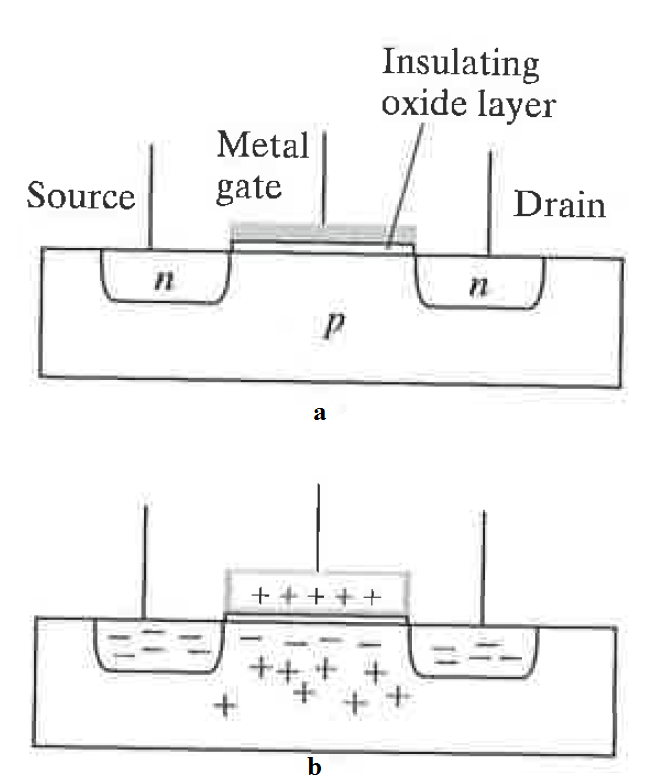
\includegraphics[scale=.45]{mosfet.png}}
\caption{ a) is a normal MOSFET without any applied charge and thus acts an npn semiconductor and does not let current flow. b) The positive charge on the metal gate cause electrons to build up along the oxide layer/semiconductor interface between the two n drops. This causes the semiconductor to turn into a n type semiconductor which allows current to flow.}
\label{mosfet}
\end{figure}

What is used to store bits is called the floating gate transistor. It is the same as the MOSFET except instead of only having one gate above the insulating oxide, you have another layer of insulating oxide on the other side of the gate followed by another gate called the control gate. So now the middle gate, also known as the floating gate, is electrically isolated due to the oxide layer on each side. Because of this, the only way to add and remove charge is through quantum tunneling. This means that when positive charge is stored on this gate as in Fig \ref{mosfet}b, current will be able to flow from the source to the drain, which corresponds to a 1. Since the charges on the floating gate can not leave it without tunneling, that means that even when the transistor is not powered, it will still store its memory. 

One method used to increase storage density is to change from using single level cells (SLC) to multi level cells (MLC). SLC is the standard floating gate where it either outputs a 1 or 0 by dividing the gate into two possible states, current or no current. However, the MLC stores 2 bits instead of one by dividing the gate into 4 possible states. While this has the benefit of doubling the storage density, it allows more room for error since the states are smaller and more difficult to distinguish. The oxide layer that was being used previously degraded after certain number of uses, and this degradation would become more visible on MLC drives first because they have to be able to distinguish states more often than SLC. However, advancements in both the durability of the oxide layer and also dynamic mapping of memory (no one gate is used more than the other) means that this has become less of an issue. 

Currently, solid state drives with a capacity of 1 TB are being sold. Flash storage can store more data than any optical disk, but it still has not reached the capacities of hard disk drives.


\section{Magnetic Storage}
\subsection{Background}
The most popular technology used to store data is magnetic storage. Magnetic storage takes advantage of the ferromagnetic property of metals such as iron. Ferromagnetic materials are composed of small magnetic domains each with their own magnetic field. An unmagnetized ferromagnet will have these domains in random directions such that the net effect is 0 as seen in Fig. \ref{domain}a. However, if an external magnetic field is applied, these domains will align with the external field and will stay aligned even after the external field is removed as in Fig. \ref{domain}b.

\begin{figure}[H]
\centerline{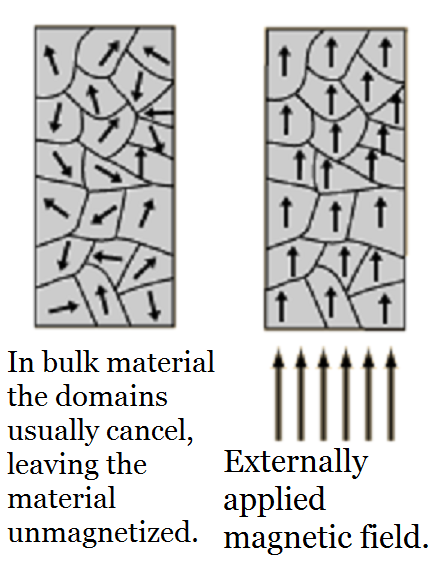
\includegraphics[scale=.55]{domains.png}}
\caption{a) An unmagnetized piece of iron where the domains are randomly oriented. b) The domains are preferentialy aligned up causing the block to be magnetized \cite{hyperDomain}.}
\label{domain}
\end{figure} 
An important phenomena that ferromagnetic materials experience is the hysteresis loop. If we start at point $a$ in Fig. \ref{hysteresis}, there is an unmagnetized ferromagnetic material with no external magnetic field. The external magnetic field, $B_0$, is increased and we get to point $b$ where there is both a noznzero external magnetic field and nonzero total field. If the external magnetic field is then decreased to zero, instead of returning to point $a$, it instead reaches point $c$. Here, even though there is no external magnetic field, there is still an internal field from the ferromagnetic material causing there to be a nonzero total field. If an external magnetic field is then applied opposite to the ferromagnetic material, point $d$ is reached where the total field ends up being 0.
\begin{figure}[H]
\centerline{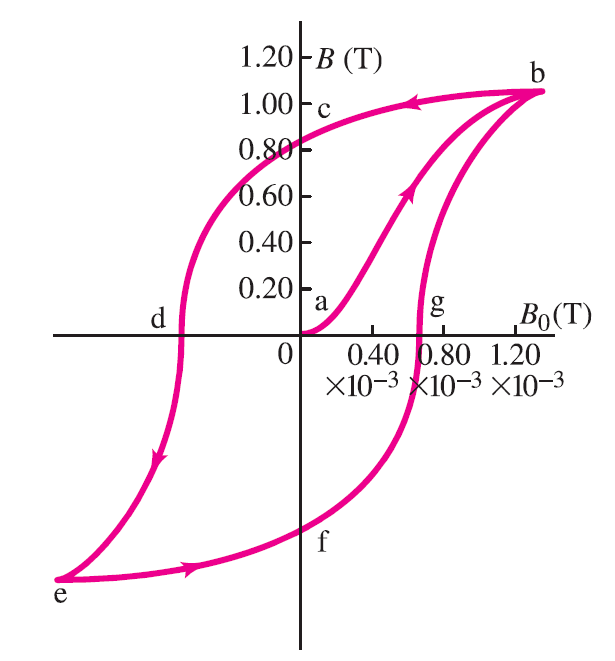
\includegraphics[scale=.4]{hysteresis.png}}
\caption{This displays a hysteresis loop of a ferromagnet. Following from point a, as an external field is applied, the total field reaches point b. As the external field is reduced to 0, since the ferromagnet partially keeps it alignment, a nonzero magnetic field exists even without an external field, point c. By applying a field in the opposite direction as before, the net field drops to zero, point d. Then applying an even stronger field will align the ferromagnet to that field reaching point e. Then to points f and g as the external field is decreased. This is important because the retainment of magnetic field by the ferromagnet means that it can store information without needing an outside, non-volatile \cite {modernPhysics}.}
\label{hysteresis}
\end{figure}
 Next, if the external magnetic field continues to increase in strength it will reach point $e$ where the ferromagnetic material aligns with the external magnetic field. Finally, if the external magnetic field is reduced to 0 again, we will reach point $f$ where there is a net field in the opposite direction of point c. This phenomenom is what allows magnetic storage to store bits. By placing a ferromagnetic material in a strong enough external magnetic field, the domains inside the material align with the external field, so when the external field is removed as in points $c$ and $f$, there is still a net magnetic field. This lingering magnetic field is what is used to store data. A bit value of 1 is read when there is a reversal of current measured meaning that the magnetic field between two domains has swapped. A bit value of 0 is read if there is no change in the magnetic field and thus no change in the direction of the current measured.
	

\subsection{Magnetic Disk Storage}
A magnetic disk drive is the most common data storage technology used in consumer products today. First introduced in 1956 by IBM, modern drives consist of of a read/write head and a hard platter with a ferromagnetic layer. Fig. \ref{basic} shows how data is recorded and read from the medium.
\begin{figure}[H]
\centerline{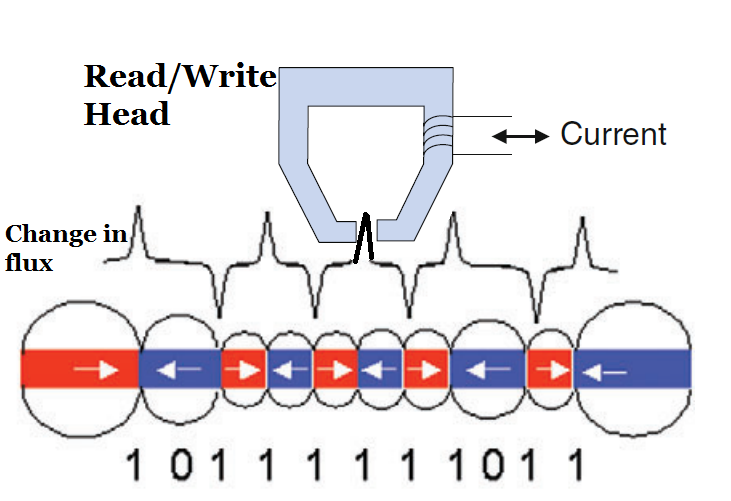
\includegraphics[scale=.55]{basic.png}}
\caption{A basic diagram of a joint read/write head with  loop of wire coiled around the head. When the head passes over a bit value of 1, two opposing domain orientations, it experiences a change in flux which induces a potential in the wire, Faraday's law, and causes a current to flow. To record data, a current is passed through the wire creating a magnetic field, Ampere's law, that aligns the domain to its field \cite{perpendicular}.}
\label{basic}
\end{figure}
Reading and writing to the material is done by inducing a magnetic field or current using a head and coil of wire. The mechanics behind this are governed by Maxwell's equations. The first relevant equation is
\begin{equation}
\oint \vec{E}\cdot \vec{ds} = -\frac{d\phi_B}{dt},
\label{faraday}
\end{equation}
which is known as Faraday's law of induction where $ \vec{E}$ is the electric field in the wire, $\vec{ds}$ is an infitesimal length of wire, $\frac{d\phi_B}{dt}$ is the change in magnetic flux \cite{purcell}. The other relevant equation is
\begin{equation}
\oint \vec{B}\cdot \vec{dl} = \mu_0 I_{enc},
\label{ampere}
\end{equation}
which is known as Ampere's law where $\vec{B}$ is the magnetic field, $\vec{dl}$ is an infitesimal length of a loop, $\mu_0$ is the permeability constant, and $I_{enc}$ is the enclosed current in the wire \cite{purcell}. Faraday's law tells us that a changing magnetic flux will induce an electromotic force (EMF) on the circuit, and Ampere's law tells us how a current through a wire generates a magnetic field. A bit value of 1 is recorded when two adjacent domains have magnetic fields in the opposite direction. This is represented as a spike or dip in the change in magnetic flux curve in Fig. \ref{basic}. A bit value of 0 is recorded when two domains have magnetic fields is in the same direction. To record data, a current is sent through the wire causing a magnetic field to form in the head due to Ampere's law. More specifically, we have a solenoid that is wrapped around the head. This generates a magnetic field parallel to the head as seen in Fig \ref{solenoid} due to the right hand rule. 

\begin{figure}[H]
\centerline{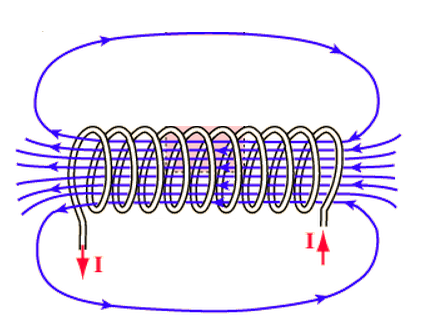
\includegraphics[scale=.8]{solenoid.png}}
\caption{A solenoid which is a coil of wire. Due to the right hand rule, all of the components of the magnetic field inside of the coil, with current flowing out of the left side, induces a magnetic field left \cite{hyperSolenoid}.}
\label{solenoid}
\end{figure}
Also, our Ampere's law equation, Eq. \ref{ampere} must be altered to account for the fact that the wire wraps around the head many times. So our new Ampere's law equation is
\begin{equation}
\oint \vec{B}\cdot \vec{dl} = \mu_0 I_{enc}N,
\label{ampere2}
\end{equation}
where N is the number of times the wire wraps around the head \cite{purcell}.
The magnetic field generated from the solenoid is then used to align the domains in a direction direction depending on the bit value desired and direction of current supplied. To read, a capacitor is attached to the wire. When the read head passes over an intersection between two domains with opposite magnetic fields, bit value 1, there is a spike in the flux read by the head. This flux spike, due to Faraday's law, applies a potential, $\oint \vec{E}\cdot \vec{ds}$  in the wire. This potential then induces a current which builds up charge on the capacitor. The presence of charge on the capacitor signifies a bit value of 1 while no charge is 0.



Originally, the head was used for both reading and writing but compromises had to be made. The read head wants a thicker gap to be better able to penetrate the medium while the write head wants a smaller gap to get better accuracy. As domains got smaller to increase density, it became more and more difficult for the read/write head to be able to properly read the intended domain due to the weaker magnetic fields sustained by the smaller domains. The discovery of the giant magnetoresistance (GMR) effect in the late 1980s brought in a new type of read head that could read weaker magnetic fields \cite{gmr}. Magnetoresistance (MR) is the property of a material to change its resistance due to an external magnetic field \cite{gmr}. However, that was limited to only a 5$\%$ change in the resistance. The GMR, however, is called giant because of its ability to change its resistance by up to 50$\%$ \cite{newGmr}. This change in resistance can be used as a more accurate way to read the bits by applying a constant potential across a giant-magnetoresistive sensor and recording how the potential changes due to the change in the resistance of the wire according to Ohm's law. 

A simplified giant magnetoresistive head can be seen in Fig. \ref{gmr2} where a nonmagnetic layer is sandwhiched by two ferromagnetic layers. One of the ferromagnetic layers is placed next to an antiferromagnetic material, not seen in Fig. \ref{gmr2}, that keeps its magnetic field aligned in one direction. This is done through something known as the exchange bias \cite{schull}. An antiferromagnet is a material that aligns anti parallel to its neighbors so it will have a net zero magnetic field. However, when above a temperature called the Neel temperature, thermal fluctuations are strong enough to destroy the magnetic ordering within the antiferromagnetic material. As seen in Fig. \ref{exchange}i, an external magnetic field is applied to the right while above the Neel temperature, so the ferromagnet (FM) aligns right while the the anti-ferromagnet (AFM) has random orientations. Then when the temperature is lowered to the neel temperature in Fig. \ref{exchange}ii, the AFM can now maintain its magnetic order and produces antiparallel spins but the ones near the interface align themselves ferromagnetically with the FM. Then in Fig. \ref{exchange}iii, when the external magnetic field is reversed, the FM tries to rotate to align itself with the external field. However, the AFM spins at the interface want to keep themselves aligned with the FM and thus applies a small torque opposing the rotation of the FM. So, a stronger external field is needed to rotate the FM than if there was no AFM attached to it. When a sufficiently strong external field does rotate the FM, the AFM still exerts a torque to rotate it back in alignment with itself, Fig. \ref{exchange} iv. So, a weaker field is needed to rotate the FM right than left implying that the FM has a prefered magnetic alignment direction \cite{schull}.


\begin{figure}[H]
\centerline{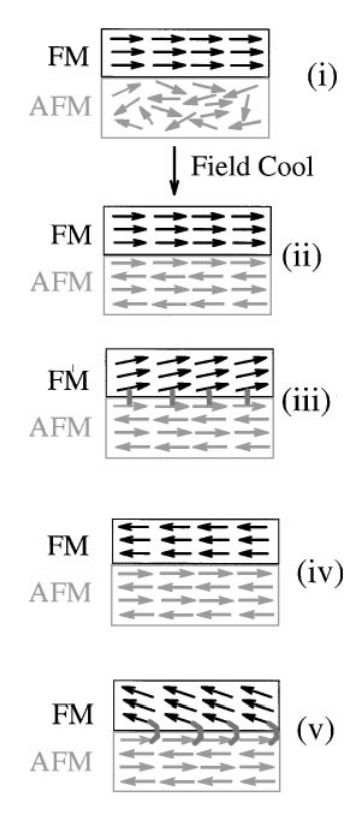
\includegraphics[scale=.55]{exchange.png}}
\caption{i) An external magnetic field is applied to the right above the Neel temperature, so the FM aligns right. ii) The temperature is lowered to the Neel temperature so the AFM orients itself antiparallel with itself and the side next to the FM parallel with it. iii) When the external magnetic field is switched to the left, the FM rotates to the left to align with it. But, the AFM wanting to stay aligned with the FM applies a torque on it to try to keep it from rotating. So a stronger external field is needed to rotate the FM than if the AFM was not there. v) After a strong enough field is applied and the FM aligned left, the AFM still tries to align with the FM applying a torque to rotate the FM right. So, a weaker external field can rotate the field right. This means that the FM has a preferred alignment to the right because of the AFM \cite{schull}.}
\label{exchange}
\end{figure}
The other ferromagnetic layer aligns itself to whatever field it reads from the hard drive. In addition, electrons are traveling through the layers horizontally. If the spin state of the electron is antiparallel to the magnetic field, it scatters and slows down. The probability of scattering depends on the number of quantum states for the electron to scatter into; since there are more states for electrons to scatter into when they are antiparallel, it occurs more \cite{gmr}. If the two ferromagnetic layers are parallel, one state of the electron spin will pass through without scattering meaning normal resistance, but if the two ferromagnetic layers become antiparallel, both states of the electron spin will scatter in one of the layers causing the resistance to increase.
\begin{figure}[H]
\centerline{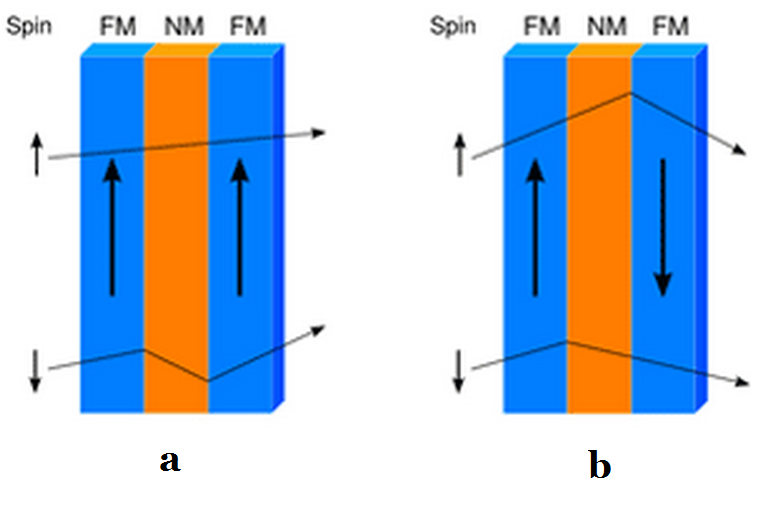
\includegraphics[scale=.55]{gmr2.png}}
\caption{The horizontal arrows represent the path of the electrons with either spin up or down as noted on the left. An angle in the path means it was scattered. The large arrows inside the FM represent the orientation of magnetic field. a) The two ferromagnetic layers are aligned causing the up spin electron to flow with out scattering and thus low resistance. b) The two ferromagnetic layers are antiparallel so both electron spins scatter in one layer causing the resistance to increase \cite{gmr}.}
\label{gmr2}
\end{figure}
The innovation of GMR read head allowed the domain sizes to shrink because the weaker magnetic fields produced by the smaller domains were still able to be read by the GMR. However, GMR allowed the magnetic field to shrink only so far. 
The ability to retain stored data in the material is true as long as 
\begin{equation}
\frac{K_uV}{k_BT} \geq 60,
\label{para}
\end{equation}
where $K_u$ is the magnetic anisotropy, $V$ is the volume, $k_B$ is boltzman's constant, and $T$ is temperature \cite{memory}. $K_u$ is proportional to how well the material can keep its aligned magnetic field. This is because after you have aligned the material along the easy axis (the axis that takes the least external magnetic field to align the material), the easier the easy axis is, and the harder it is to try to get the magnetic field to align with the hard axis. The numerator of the left side represents the energy barrier that must be overcome for the ferromagnetic material to lose its magnetic field. As the domains decrease in size to increase density, the volume decreases and so does the energy barrier. If the volume of the domain decreases to the point where Equation \ref{para} is not true, then the domain may randomly switch its field direction which would ``flip bits"; this is known as the super paramagnetic limit. This creates a limit to the storage density that longitudinal recording (i.e. magnetic field parallel to the surface of hard drive) can attain \cite{perpendicular}.

To surpass this limit, the orientation of the recorded magnetic field changed from longitudinal recording to perpendicular recording as seen in Fig. \ref{perpendicularComparison}. In addition to the change in orientation, the writing head was changed to a "mono-pole" head and a malleable soft underlayer(SUL) was added below the recording material. The permeability of the SUL allowed it to act as a mirror to the write head and directs the magnetic flux to the collector head. This increased the induced magnetic field used to write data \cite{highDensity}. The stronger magnetic field means that materials with higher anisotropy values could be used that were not feasible for the weaker magnetic field in longitudinal recording. Because the anisotropy constant can be increased, the volume of the domain can be decreased further without worrying about thermal fluctuations. With all the above innovations, current HDDs can achieve a storage density of around 500 Gb/in$^2$ and total storage of a 1 TB per drive.

\begin{figure}[H]
\centerline{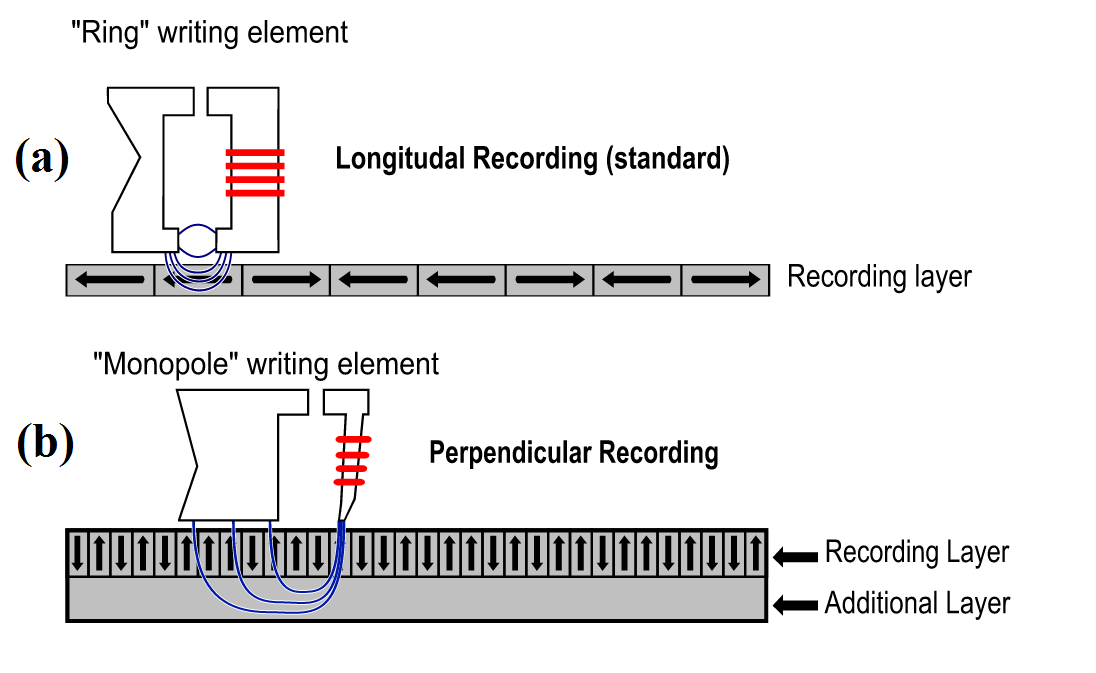
\includegraphics[scale=.45]{perpendicularComparison.png}}
\caption{Perpendicular recording due to the presence of the additional layer, soft underlayer, a much larger magnetic field can be applied to the recording layer. This allows us to use material with higher anisotropy meaning the domain size can be reduced and density increased.}
\label{perpendicularComparison}
\end{figure}


However, this too will have a limit at a smaller domain size where thermal fluctuations will be an issue again. One method still in development is called heat-assisted magnetic recording (HAMR). This method is based on the fact that all ferromagnetic materials have a curie temperature where the internal magnetic field the material had is lost and aligns itself to any external magnetic field. In HAMR, when a bit needs to get written to, a laser is used to heat up the desired domain to the curie temperature allowing the magnetic field generated by the write head to align the domain, and then allowing the material to cool back down. This means that the recording material can be changed to one with a much higher anisotropy value allowing the domain sizes to decrease even more, further increasing the storage density to around 1 Tb/in$^2$ \cite{hamr}. 

While the technique of storing data in magnetic fields is old, new techniques are applied to further the life of HDDs. Now, HDDs are the most dense and have the largest capacity drives of the previous two techniques with HAMR drives soon to be released with 2 TB of storage \cite{seagate}.


\section{Future Technology}

While the previous three techniques are already established, we need to look into other techniques to store data as the world creates more and more of it. One of these new techniques still in development is holographic data storage (HDS), which has the potential to store over 1Tb/in$^2$ \cite{HDS}. In the most basic sense, holography is the method of capturing and recreating optical information through interference patterns. A hologram then is a recording of an interference pattern. Fig. \ref{create} shows how to record a hologram. 

\begin{figure}[H]
\centerline{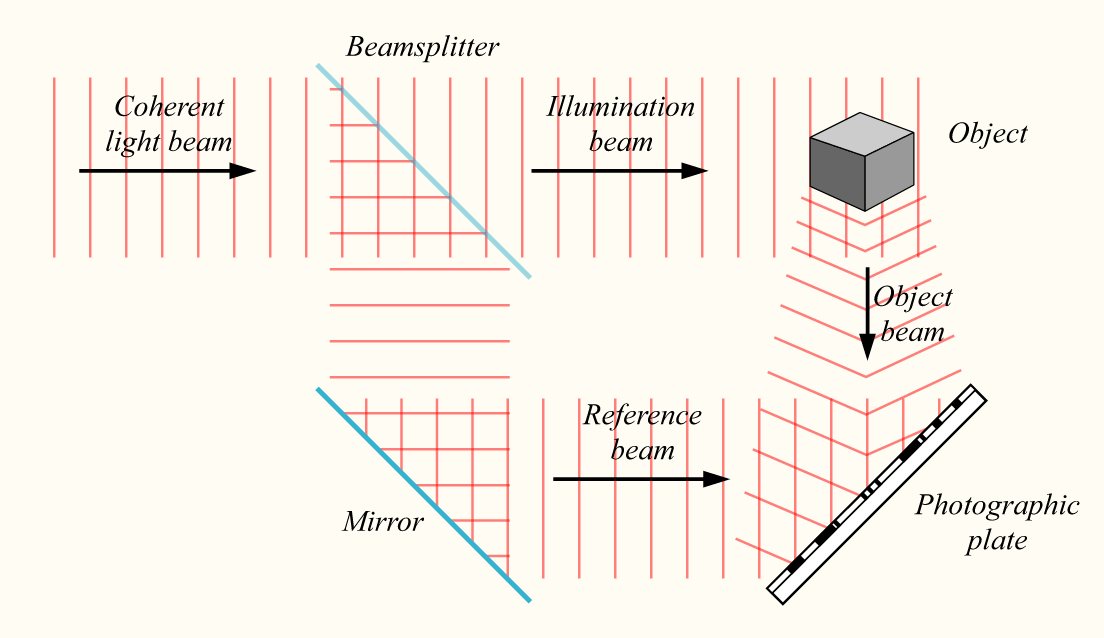
\includegraphics[scale=.5]{create.png}}
\caption{This is an example of a transmission hologram where a coherent souce of light is split into a reference beam and an object beam. The two beams create an interference pattern at the photographic plate creating regions of constructive and destructive interference which is recorded onto the hologram \cite{wikiHolo}.}
\label{create}
\end{figure} 
First a coherent light source is split into a reference beam, $E_R$ and object beam, $E_O$, using a beam splitter where $E_R$ is

\begin{equation}
E_{R} = re^{i(\omega t + \phi)},
\label{eRef}
\end{equation}
where $r$ is the amplitude of the beam and is assumed to be constant over the surface of the film due to the plane wavefront of the reference beam, $\omega$ is the angular frequency, and $\phi$ is the phase angle that relates to the tilt of the photographic plate relative to the reference beam wavefront and varies with $x$ by $(\frac{2\pi}{\lambda}xsin\alpha$, as seen in Fig. \ref{eRefMath}. $\Delta$ is the extra distance traveled by certain parts of the wavefront depending on the angle of the beam relative to the normal when the top border of the beam hits the plate at x = 0 \cite{optics}.

\begin{figure}[H]
\centerline{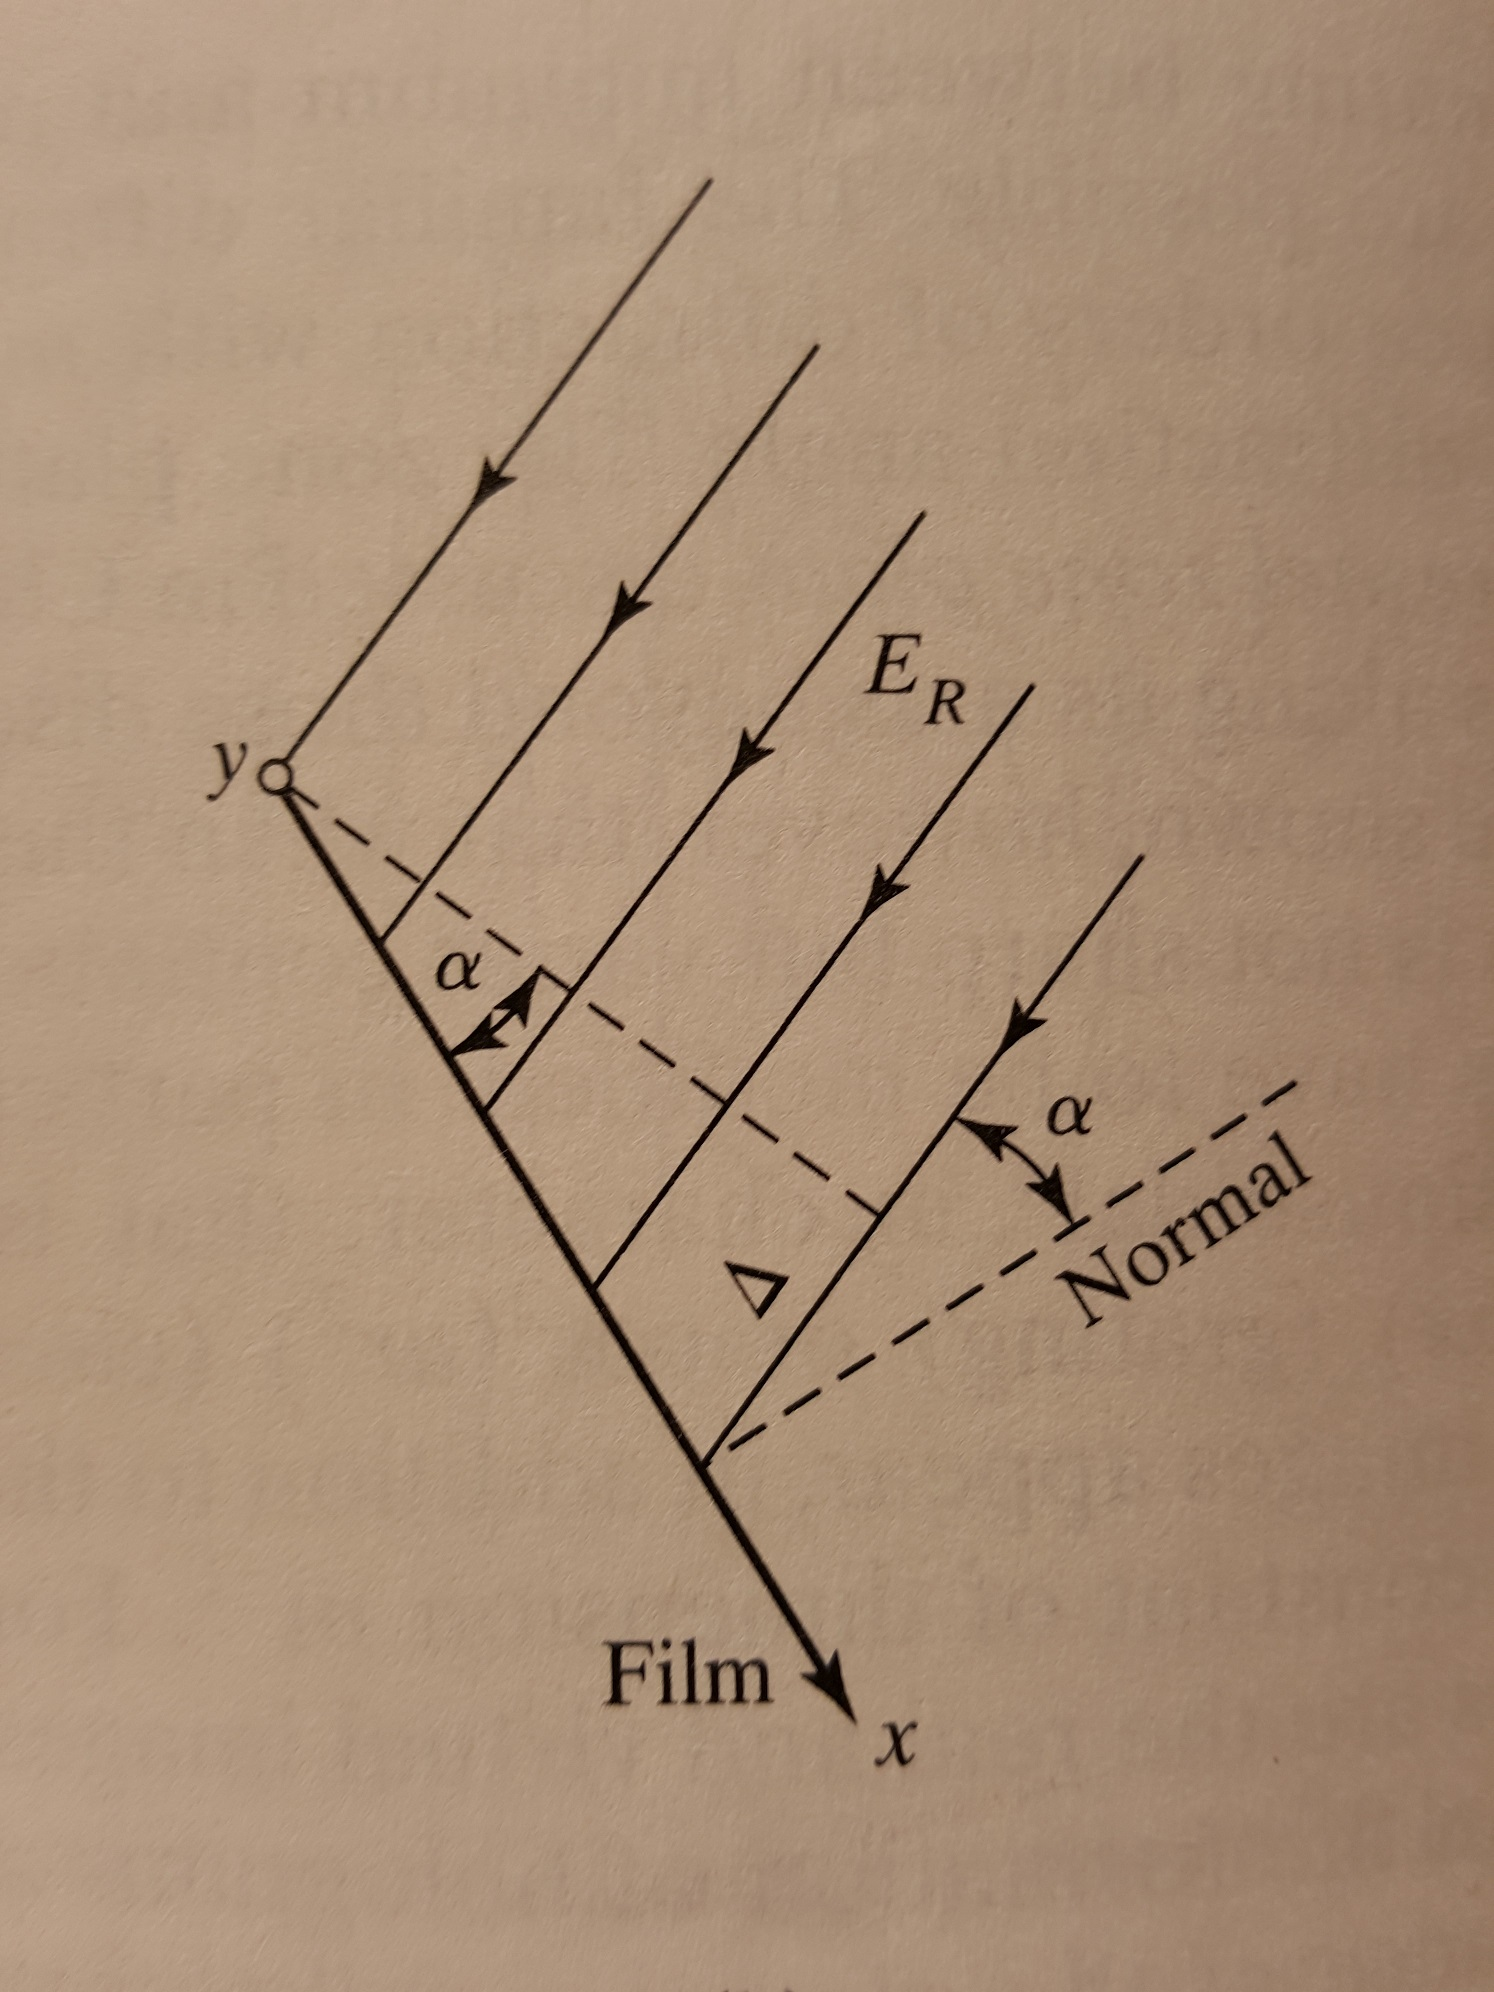
\includegraphics[scale = .17]{eRefMath.jpg}}
\caption{The intersection of the reference beam and the photographic film \cite{optics}.}
\label{eRefMath}
\end{figure} The object beam is reflected off the object being recorded and is incident on the photographic plate. The object beam, $E_O$ can be represented by,
\begin{equation}
E_{O} = oe^{i(\omega t + \theta)},
\label{eObj}
\end{equation}
where $o$ is the amplitude of the reflected light off the object, and $\theta$ is analogous to $\phi$ except that it is more complicated due to variations in the phase of the light because it is reflected from different parts of the object \cite{optics}. The reference beam, also being shone on to the photographic plate, interferes with the object beam and that interference pattern is recorded on the plate as a hologram. Destructive interference appears as darker spots and constructive interference appears as brighter spots. 
The resultant electric field at the plate, $E_P$ is given by
\begin{equation}
E_{P} = E_R + E_O.
\label{Ef}
\end{equation}

The quantity that describes the hologram is known as scaled irradiance which is Eq. \ref{iInf} without the constants in the front. Thus, the scaled irradiance at the plate is
\begin{equation}
I_{P} =  |E_P|^2 = (E_R + E_O) (E^*_{R} + E^*_{O}),
\label{If}
\end{equation}
where the asteriks represent the complex conjugate form of the variable.
By multiplying the binomials and subbing in for $E_R$ and $E_O$ from Eqs \ref{eRef} and \ref{eObj}, respectively, $I_P$ can be simplified to \cite{optics}
\begin{align}
\begin{split}
I_{P} &= r^2 + o^2 + E_O E^*_R + E_R E^*_O  \\
I_{P} &= r^2 + o^2 + roe^{i(\theta - \phi)} + roe^{-i(\theta - \phi)}.
\end{split}
\label{IfFinal}
\end{align}

To recreate the image from the hologram, the reference beam in Fig. \ref{reconstruct} is shone back at the hologram at the same angle and by looking at where the object should be through the hologram, a virtual image can be seen of the object. This is due to the reversibility of light which states that light will take the same path if the direction it travels is reversed. So when we shine the reference beam through the hologram and view it with our eyes, our eyes trace the light back the same path it took when the hologram was created with the object beam and we see a virtual image.

\begin{figure}[H]
\centerline{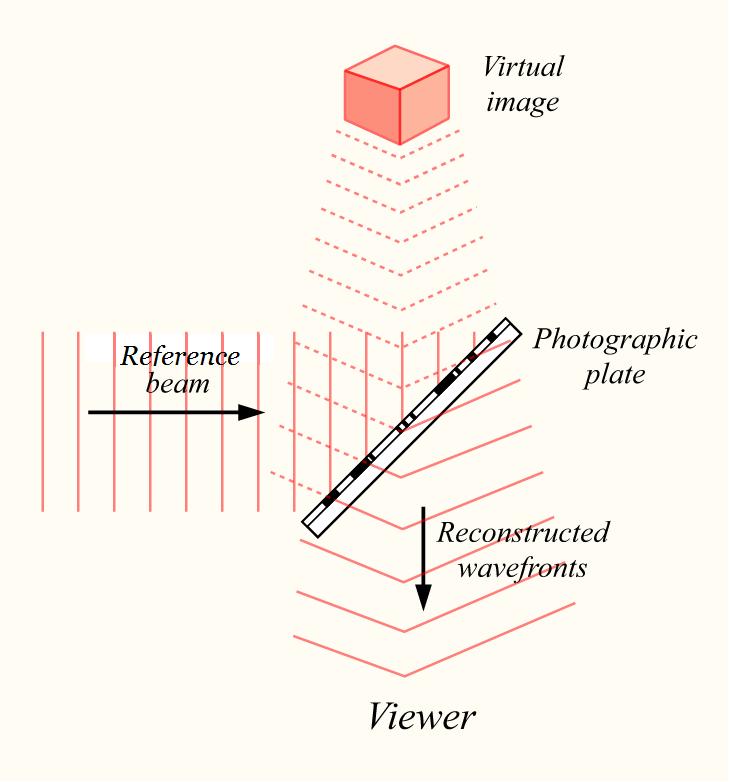
\includegraphics[scale=.45]{reconstruct.png}}
\caption{To recreate the virtual image, the reference beam is shined on the hologram at the same angle, and by looking through the hologram to where the object should be, a virtual image can be seen \cite{wikiHolo}.}
\label{reconstruct}
\end{figure} 
Mathematically, the recreation of the image using the hologram by shining the reference beam is given by,
\begin{equation}
E_H =  I_P E_R = (r^2 +s ^2)E_R + r^2oe^{i(\omega t +\theta)} + r^2e^{i(2\phi)}e^{i(\omega t-\theta)}.
\label{Eh}
\end{equation}
The first term of $E_H$ is identical to Eq \ref{eRef} except that it is multiplied by $r^2$. Thus the first term represents an amplitude modulated (amplitude and thus irradiance changed) version for the reference beam. The second term in $E_H$ is identical to Eq \ref{eObj} except by a multiplfication factor and thus we get the amplitude modulated object beam This is the virtual image viewed as the hologram and is a virtual image since no light is present at the image, rather it is created due to our eye reversing the light back to the image. The last term is the similar to Eq \ref{eObj} except there is a constant factor being multiplied and $e^{i\theta}$ is changed to $e^{-i\theta}$ which represents the amplitude and phase modulation respectively. The phase delay in the third term of Eq \ref{Eh} shows up as a phase advance, so the image is turned inside out and is real \cite{optics}. 

Moving on, holograms can be created in both thick and thin regimes. The thin regime is unsuitable for high density storage because thin holograms like those written on photographic film confine their diffractive interaction to a single plane and can not be used for multiplexing \cite{HDS}. The criteria used quantify the thickness or thinness of a hologram is known as the $Q$ parameter. The $Q$ parameter is given by 
\begin{equation}
Q = \frac{2\pi\lambda L}{n_0\Lambda^2},
\label{qParameter}
\end{equation}
where $\lambda$ is the wavelength of the light, $L$ is the thickness of the recording layer, $n_0$ is the index of refraction of the medium, and $\Lambda$ is the grating period. A hologram is considered in the thin regime if $Q<1$ and is considered in the thick regime if $Q>1$. $L$ can range from 500$\mu$m to a few millimeters \cite{HDS}.

To store digital data in holograms, a spatial light modulator (SLM) is needed. The SLM converts the 1s and 0s of the digital data into light and dark pixels respectively onto a 2D image called a page. The number of bits that can be stored per SLM image can be over one million, but this varys with the SLM's pixel count. So to record digital data, instead of reflecting the object beam off of the object, it is shone through the SLM then onto the storage medium as seen in Fig. \ref{dataHologramCreate}. 

\begin{figure}[H]
\centerline{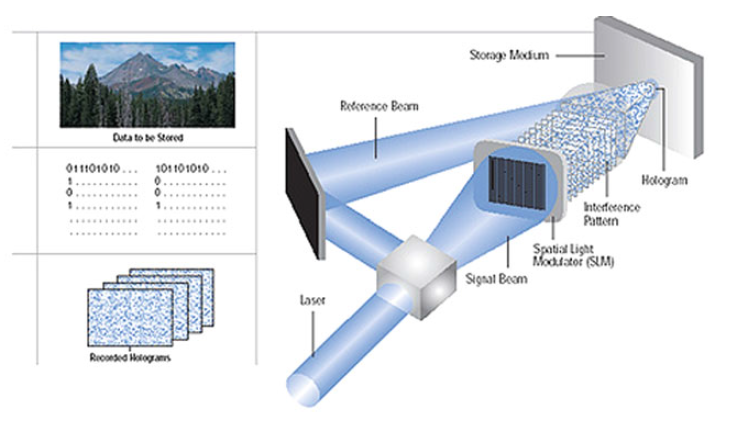
\includegraphics[scale=.45]{dataHologramCreate.png}}
\caption{This implementation of holographic storage uses the same technique as a transmission hologram except instead of reflecting the object beam off of the object, it is shone through the SLM which contains the bit information. Since the SLM page contains many bits at once, it can write more than one bit at once unlike magnetic drives  \cite{HDS}.}
\label{dataHologramCreate}
\end{figure} 
To read, the reference beam is shone at the hologram, but now there is a detector array to convert the SLM's image of dark and bright spots into 1s and 0s for the computer.
\begin{figure}[H]
\centerline{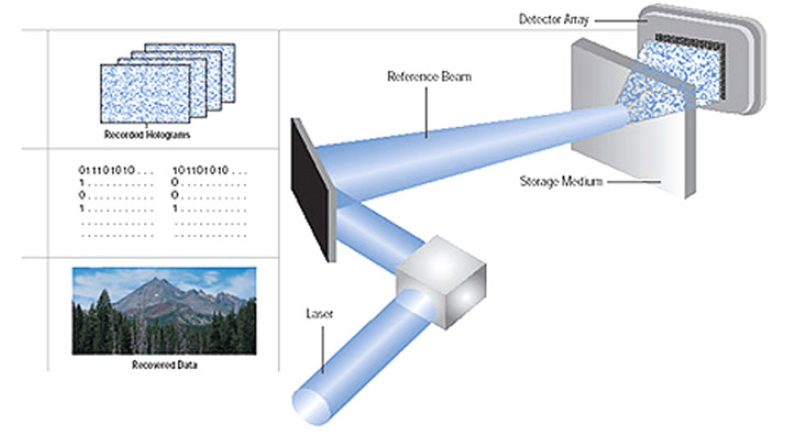
\includegraphics[scale=.45]{dataHologramReconstruct.png}}
\caption{Reading information is the same as recreating a hologram except now the virtual image is shone onto a detector array which converts the dark and bright spots into 1s and 0s  \cite{HDS}.}
\label{dataHologramReconstruct}
\end{figure} 
The reason why HDS can be so dense is because of its ability to superimpose holograms in the same volume; this is known as multiplexing. HDS offers many different methods for multiplexing. One category of multiplexing methods is known as Bragg-Based techniques which rely on the Bragg condition. Since the angle of the reference beam must match the angle it had when recording the hologram, that means that a small change in the angle when recreating the image will cause the image to not appear sharply or at all. We can use this sensitivity by having one page of data from the SLM stored at one angle and another page in the same volume by changing the angle of entry. Specifically, the spacing between the diffraction max and the first diffraction min, angular selectivity, is given by
\begin{equation}
\Delta \theta = \frac{\lambda cos\theta_o}{Lsin(\theta_r + \theta_o)},
\label{angular}
\end{equation}
where $\theta_r$ and $\theta_o$ are the reference and object angles and $L$ is the media thickness \cite{HDS}. To minimize noise and interference between different pages, each page would have its Bragg peak at the null position in the diffraction efficiency of every other page by changing the reference angle by multiples of the angular selectivity. A similar method to add multiplexing is to vary the wavelength of the the source and reference beams. This method is limited due to the small tuning range of lasers. Yet another method is to vary the point of entry of the beams into the medium. While there are more methods of multiplexing, the true benefit of multiplexing occurs when combining multiple multiplexing techniques at once. For example, hybrid wavelength and angular multiplexing systems have been tested before \cite{memory}. However, HDS is very much still in development with the only commercialized product only having a capacity of 300 GB. Nevertheless, it still is a possible candidate for storing our data in the future.

\section{Conclusion}
Digital data storage allows us to store our digital information in a variety of different methods. We are already able to store data at incredible densities or speeds, but as more and more information is being saved digitally we will need denser and larger capacity devices. Since only two states are needed to store memory, it is very easy to find techniques to store memory like punch cards. However, it is quite difficult to find techniques that are dense and efficient. As we have seen, there is continued improvements being made to current data storage techniques such as Blu-Ray disks and HAMR in hard drives. However, these are only short term solutions to our storage needs. Holographic storage is a new techniques that could be useful, but it is still only in development. As our data needs keep growing, the technology needed to support that will continue to evolve as well.


\section{Acknowledgements}
I would like to thank my comps advisors Professor Marty Baylor, Professor Nelson Christensen, and Leah Crane. I would also like to thank the Carleton College physics department for supporting me the past 4 years.

\bibliographystyle{aip}
\bibliography{myCollection2}
\newpage

\begin{appendices}
\chapter{Appendix}
\begin{figure}[H]
\centerline{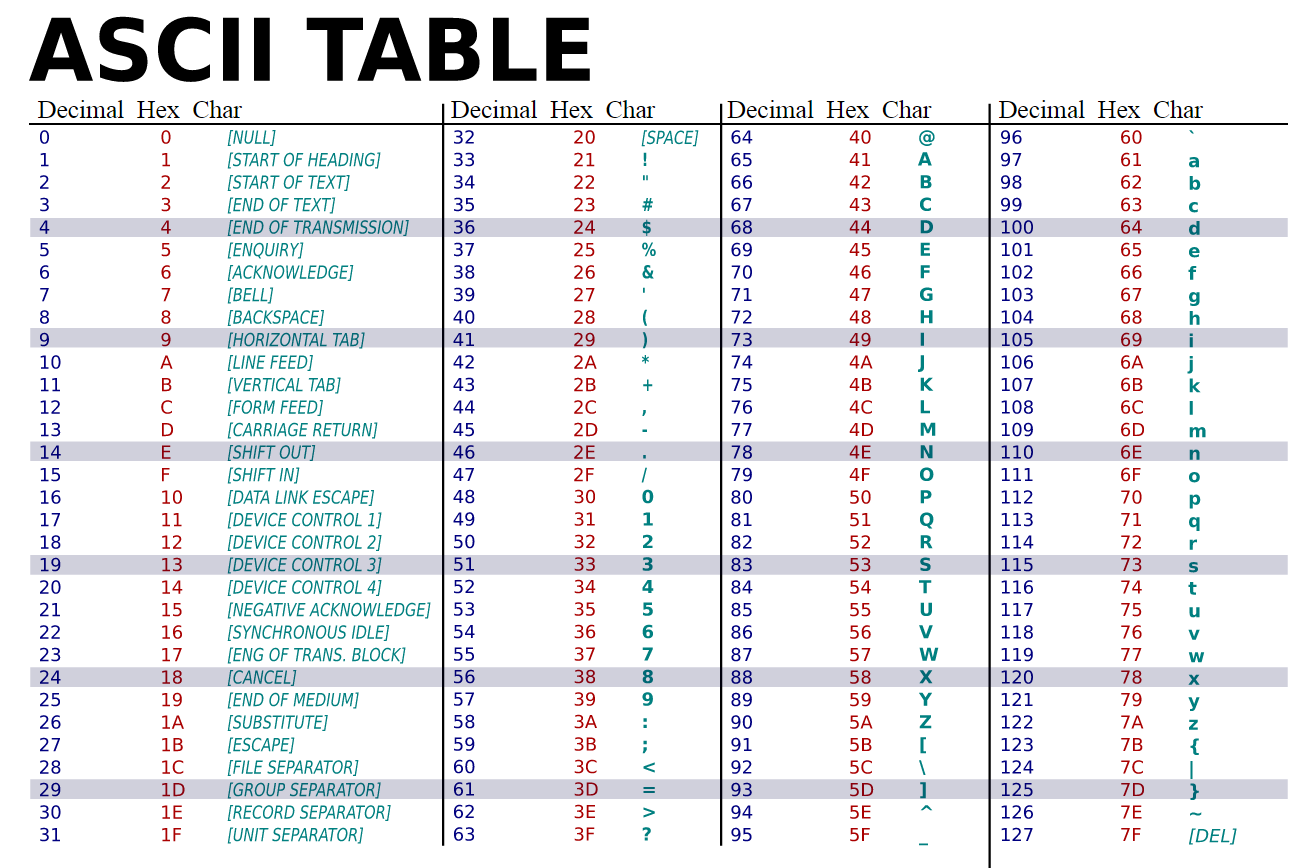
\includegraphics[scale=.45]{ascii.png}}
\end{figure} 
\end{appendices}
\end{document}

